
%(BEGIN_QUESTION)
% Copyright 2006, Tony R. Kuphaldt, released under the Creative Commons Attribution License (v 1.0)
% This means you may do almost anything with this work of mine, so long as you give me proper credit

Graph the output of this proportional-only controller, assuming a proportional band value of 40\%, a constant setpoint, and a control action that is direct-acting:

$$\includegraphics[width=15.5cm]{i01500x01.eps}$$

\vskip 20pt \vbox{\hrule \hbox{\strut \vrule{} {\bf Suggestions for Socratic discussion} \vrule} \hrule}

\begin{itemize}
\item{} Explain how it is possible to sketch an output trend without knowing the setpoint or bias values for this controller.
\end{itemize}

\underbar{file i01500}
%(END_QUESTION)





%(BEGIN_ANSWER)

$$\includegraphics[width=15.5cm]{i01500x02.eps}$$

%(END_ANSWER)





%(BEGIN_NOTES)

With a proportional band value of 40\%, the gain will be equal to 2.5.  This means any change in PV will result in the output changing 2.5 times as much.

% No blank lines allowed between lines of an \halign structure!
% I use comments (%) instead, so that TeX doesn't choke.

$$\vbox{\offinterlineskip
\halign{\strut
\vrule \quad\hfil # \ \hfil & 
\vrule \quad\hfil # \ \hfil \vrule \cr
\noalign{\hrule}
%
% First row
{\bf PV} & {\bf Output} \cr
%
\noalign{\hrule}
%
% Another row
45\% & 25\% \cr
%
\noalign{\hrule}
%
% Another row
70\% & 87.5\% \cr
%
\noalign{\hrule}
%
% Another row
65\% & 75\% \cr
%
\noalign{\hrule}
%
% Another row
55\% & 50\% \cr
%
\noalign{\hrule}
%
% Another row
50\% & 37.5\% \cr
%
\noalign{\hrule}
} % End of \halign 
}$$ % End of \vbox


%INDEX% Control, proportional: graphing controller response

%(END_NOTES)


